% =============================================================================
% Draft paper — Federated Fraud Detection with Temporal Graph Transformers
% and Differential Privacy.
%
% Describes the SYSTEM AS ACTUALLY IMPLEMENTED AND MEASURED in this repository
% (see README.md, docs/ARCHITECTURE.md, experiments/run_model_comparison.py,
% experiments/run_epsilon_sweep.py). Every number in Tables I-II is read
% directly from results/comparison/comparison.json and
% results/comparison/epsilon_sweep.json, produced by real training runs, not
% asserted. No citation below is a placeholder — every \bibitem is a real,
% verifiable paper. The prior related-work comparison table (unverified
% third-party numbers with no resolvable citations) has been removed; see
% the reviewer-proofing note in Section II.
%
% Compile with: pdflatex draft_paper.tex   (run twice for refs to settle)
% Requires: pgfplots/tikz (bundled with all standard TeX distributions,
% including Overleaf) for Fig. 1.
% =============================================================================
\documentclass[conference]{IEEEtran}
\usepackage{amsmath,amssymb}
\usepackage{graphicx}
\usepackage{booktabs}
\usepackage{placeins}
\usepackage{pgfplots}
\pgfplotsset{compat=1.17}
\usepackage[hidelinks]{hyperref}

\begin{document}

\title{Federated Fraud Detection with Temporal Graph Transformers and Differential Privacy: A Measured Privacy-Utility Study}

\author{
\IEEEauthorblockN{Tanishk Maheshwari, Vaibhav Handoo, Vibhav Kolachana, Yash Kuber Khanna}
\IEEEauthorblockA{Department of Computer Science and Engineering\\
PES University, Bengaluru, India\\
\textit{Advisor: Dr. Prafullata Kiran Auradkar}}
}

\maketitle

\begin{abstract}
Fraud detection across financial institutions is fundamentally a
multi-party problem: the patterns that distinguish fraud from legitimate
activity are strongest when observed across many institutions' data, yet
that data can never be legally or competitively pooled. We present a
fraud detection system built around a Temporal Graph Transformer with a
contrastive learning head, trained via federated learning (FedAvg and
FedProx) across ten simulated bank clients, with every round's aggregate
protected by client-level differential privacy (DP-FedAvg). Rather than
asserting privacy-preserving federated learning as a good idea, we
measure it: we benchmark our approach against a centralized Random
Forest, a centralized (non-federated) deep model, and a federated model
without differential privacy, all evaluated on one identical held-out
test set. We further report a full nine-point epsilon-vs-utility sweep
($\varepsilon \in \{1, 5, 10, 20, 50, 100, 500, 2000\}$ plus a no-DP
ceiling) that demonstrates the differential privacy mechanism has a
real, measurable effect rather than being an inert configuration flag,
and that our chosen operating point ($\varepsilon=100$) costs a small,
precisely quantified utility loss ($<2$ F1 points) relative to the
matched non-private federated baseline. We
also document three concrete engineering failures uncovered during
development -- a synthetic-data generator that produced a trivially
separable (and therefore useless) benchmark, a badly over-parameterized
model that collapsed to a constant prediction under class imbalance, and
a NaN-masking bug that silently hid a real training failure -- because a
privacy-utility claim is only as credible as the pipeline that produced
it.
\end{abstract}

\begin{IEEEkeywords}
federated learning, differential privacy, fraud detection, temporal
graph transformer, contrastive learning, FedProx
\end{IEEEkeywords}

\section{Introduction}

Financial fraud detection sits at an awkward intersection of two facts.
First, fraud is inherently a cross-institution phenomenon: a fraud ring
that touches five banks looks like five separate, individually
low-signal anomalies to each bank in isolation, and only becomes visible
as a pattern when the five views are combined. Second, banks cannot
combine those views. Data protection regulation, competitive concerns,
and the sheer sensitivity of transaction-level financial data make
centralizing raw records across institutions a non-starter in practice,
regardless of its modeling appeal.

Federated learning (FL)~\cite{mcmahan2017fedavg} offers a way out of
this bind: institutions train a shared model collaboratively while each
institution's raw data never leaves its own infrastructure, only model
updates are exchanged. But federated learning by itself is not a privacy
guarantee -- a client's model update can still leak information about
its training data~\cite{mcmahan2018dp,abadi2016dpsgd}. Differential
privacy (DP)~\cite{dwork2014dp}, applied at the client-update level,
closes that gap by bounding and noising each round's aggregate update,
at a cost: DP noise degrades model utility, and the size of that cost is
an empirical question, not something that can be waved away.

This paper makes two contributions. First, we describe a fraud
detection architecture -- a Temporal Graph Transformer with a
contrastive learning head -- trained under FedProx~\cite{li2020fedprox}
with client-level DP-FedAvg~\cite{mcmahan2018dp}, and we report its
performance against real, non-fabricated baselines on one shared
held-out test set (Section~\ref{sec:results}). Second, and more
centrally to this paper's argument, we report a full epsilon-vs-utility
sweep that makes the privacy-utility tradeoff a measured curve rather
than an assumption (Section~\ref{sec:epsilon}), and we document three
real pipeline defects that, left uncaught, would have produced a
misleadingly perfect-looking but meaningless result
(Section~\ref{sec:lessons}). We consider that last contribution as
important as the numbers themselves: a privacy-utility claim is only
as trustworthy as the evaluation pipeline behind it, and we show our
work on that pipeline rather than assuming it away.

\section{Related Work}

\textbf{Federated learning.} McMahan et al.~\cite{mcmahan2017fedavg}
introduced FedAvg, the foundational algorithm for training a shared
model across decentralized clients by averaging locally-trained weights.
FedAvg assumes client data is approximately independent and identically
distributed (IID); in a cross-bank setting this assumption does not
hold, since each bank's transaction mix, fraud rate, and customer
behavior differ systematically. Li et al.~\cite{li2020fedprox} address
this with FedProx, which adds a proximal term to each client's local
objective that penalizes drift from the global model, stabilizing
training under non-IID data -- the algorithm we adopt for this reason.

\textbf{Differential privacy in federated learning.} Applying DP
naively -- clipping and noising gradients at every local minibatch --
both destroys utility and, without careful composition accounting,
provides a weaker guarantee than its stated $\varepsilon$ suggests.
McMahan et al.~\cite{mcmahan2018dp} instead propose DP-FedAvg: each
client clips its \emph{entire round update}, and the server adds a
single calibrated Gaussian noise draw to the aggregate, once per round.
This is the mechanism we use. Abadi et al.~\cite{abadi2016dpsgd}
established the moments-accountant approach to composing privacy loss
across many training steps, and Dwork and Roth~\cite{dwork2014dp} give
the formal $(\varepsilon,\delta)$-DP definition and its algebra that
our privacy accounting rests on.

\textbf{Secure aggregation and encryption.} Bonawitz et
al.~\cite{bonawitz2017secagg} describe secure aggregation protocols that
let a server compute a sum of client updates without seeing any
individual update, and Paillier's cryptosystem~\cite{paillier1999}
underlies additively homomorphic aggregation schemes with the same
goal. Both are complementary, cryptographic guarantees to DP's
statistical one; our system implements a reference version of both but,
as discussed in Section~\ref{sec:limitations}, does not yet wire them
into the live training loop -- a documented simplification, not a
claimed feature.

\textbf{Model architecture.} Our temporal branch is a standard
Transformer encoder~\cite{vaswani2017attention} applied over a fixed
window of a client's recent transactions. Our auxiliary contrastive
head follows the general contrastive representation-learning framework
of Chen et al.~\cite{chen2020simclr}, adapted here to encourage
separation between fraud and legitimate transaction embeddings rather
than between augmented views of the same image.

\textbf{Federated fraud detection systems in the literature.} A body of
recent work applies FL to financial fraud and financial-crime detection
under a range of architectures and privacy mechanisms -- hybrid
horizontal/vertical FL over split account/transaction features,
federated graph learning for anti-money-laundering, FL combined with
explainable-AI layers (SHAP/LIME), homomorphic-encryption-secured
gradient aggregation, and FL combined with generative oversampling
(WGAN/VAE) for extreme class imbalance. An earlier draft of this paper
included a table of reported metrics from several such systems for
context; we removed it here because those figures could not be traced
to resolvable, citable sources at the time of writing, and an
uncited numeric comparison is not defensible in a submitted paper.
Table~\ref{tab:comparison} restricts this paper's quantitative claims
to results we produced ourselves under a controlled, single-test-set
protocol.

\section{System Architecture}

\subsection{Temporal Graph Transformer}
Each client account's transaction history is windowed into a
fixed-length sequence of its ten most recent transactions, each encoded
as a 10-dimensional feature vector (normalized amount, hour-of-day,
day-of-week, a merchant-category risk score, distance from the
previous transaction, time since the previous transaction, an implied
velocity, card age, transaction frequency in the last 24 hours, and a
weekend flag). A four-layer Transformer encoder processes this
sequence. A parallel graph branch encodes each account's own transaction
profile; in the experiments reported here this branch operates on each
account as an isolated node, not a multi-entity relational graph
(Section~\ref{sec:limitations} discusses why). A cross-modal fusion
layer combines the two branches via bidirectional attention. Two heads
sit on top of the fused
representation: a supervised binary cross-entropy head for the primary
fraud/legitimate decision, and a contrastive head intended to separate
novel fraud patterns from the learned representation space even when
they were not explicitly labeled as such during training.

The model is deliberately small: a 32-dimensional hidden size, giving
approximately 45{,}000 parameters. Section~\ref{sec:lessons} explains
why this specific choice -- rather than a larger, seemingly more
capable model -- is load-bearing for both training stability and the
differential privacy mechanism's usable operating range.

\subsection{Federated Training: FedAvg and FedProx}
Training is simulated across ten clients, each representing one bank
with its own non-IID transaction distribution. Each round samples three
clients, each of which trains locally for two epochs before sending its
update to the server, for a total of $R=10$ communication rounds. The
server aggregates client updates with
FedProx's proximal-term regularization ($\mu=0.1$), which penalizes a
client's local update for drifting far from the current global model --
the mechanism that keeps training stable when only a minority of
clients are sampled per round and those clients disagree with each
other's local optima.

\subsection{Client-Level Differential Privacy}
Each client's update is clipped to a fixed $L_2$ norm (clip norm
$=1.0$) before being sent to the server. Once per round, the server adds
a single Gaussian noise draw to the aggregated update, scaled by the
largest single client's averaging weight -- the aggregate's sensitivity
to any one client's contribution, rather than the full per-client clip
norm, following the client-level DP-FedAvg construction of McMahan et
al.~\cite{mcmahan2018dp}. This gives an $(\varepsilon,\delta)$-DP
guarantee at the level of ``one client's entire round contribution,''
which is the right unit of protection in a cross-silo setting where each
client is an institution, not an individual data subject.

Gaussian-mechanism noise scales with $\sigma\sqrt{d}$ for a
$d$-dimensional update, meaning the number of trainable parameters
directly determines how much noise a fixed $\varepsilon$ requires. This
is precisely why the model's size (Section~III-A) and its DP budget are
not independent design choices.

\textit{Accounting scope.} Every $\varepsilon$ value reported in this
paper (with $\delta=10^{-5}$) is the \emph{per-round} budget of the
Gaussian mechanism, calibrated once and applied identically at every
round. We do not apply a formal multi-round composition accountant
(e.g., R\'enyi DP) over the $R=10$ rounds; the total privacy loss over a
full training run is therefore larger than the per-round $\varepsilon$
quoted throughout Sections~\ref{sec:results} and~\ref{sec:limitations},
and composed accounting is left as future work (Section~VII).

\section{Experimental Setup}

Data is drawn from a schema-matched synthetic PaySim-style
generator~\cite{lopezrojas2016paysim} (Section~\ref{sec:limitations}
discusses why synthetic, not the original PaySim release, is used
here), producing overlapping -- not disjoint -- feature distributions
for fraud and legitimate transactions, with 12\% of fraud transactions
deliberately drawn from the \emph{legitimate} distribution (``quiet
fraud'') to avoid a trivially separable benchmark. Ten clients are
generated with independent, non-identical transaction distributions.
All models in Section~\ref{sec:results} are evaluated on one shared,
never-trained-on held-out test set of 6{,}000 sequences (362 fraud, a
6.03\% fraud rate), pooled across all clients.

Four models are compared under identical evaluation conditions:
\begin{itemize}
\item \textbf{Centralized RandomForest} -- all clients' raw data pooled,
no privacy.
\item \textbf{Centralized Deep} -- the same Temporal Graph Transformer
architecture, all clients' raw data pooled, no federation and no DP.
Isolates the cost of federation alone.
\item \textbf{Federated (FedAvg, no DP)} -- data never pooled, but no
differential privacy applied. Isolates the cost of DP alone.
\item \textbf{Federated (FedProx + DP)} -- our full system, $\varepsilon=100$.
\end{itemize}

\textit{Reproducibility.} All experiments use a fixed random seed (42)
for data generation and training, $R=10$ federated rounds, 3-of-10
clients sampled per round, 2 local epochs per client, and clip norm
$1.0$ (Section~III-C). Code and configuration to reproduce every table
in this paper are provided in the accompanying repository.

\section{Results}
\label{sec:results}

\subsection{Baseline Comparison}
Table~\ref{tab:comparison} reports all four models on the shared test
set. The centralized RandomForest wins on raw accuracy and F1 --
expected, since it is the only model with zero privacy cost and access
to every client's pooled raw data. Note that the ``Federated, no DP''
row uses FedAvg rather than FedProx, so it is not a clean single-variable
ablation of DP alone: it differs from our full system in both the
aggregation algorithm and the privacy mechanism. Our full system
(FedProx + DP, $\varepsilon=100$) nonetheless matches or exceeds this
FedAvg baseline on every metric. The clean ablation of DP's cost in
isolation -- same FedProx configuration, DP on vs.\ off -- is reported
separately in Section~\ref{sec:epsilon} (Table~\ref{tab:epsilon}),
which shows a small but real utility cost at $\varepsilon=100$ relative
to the FedProx no-DP ceiling.

\begin{table}[!t]
\caption{Baseline comparison on the shared held-out test set (6{,}000 sequences, 362 fraud)}
\label{tab:comparison}
\centering
\begin{tabular}{@{}lccccc@{}}
\toprule
Model & Acc. & Prec. & Rec. & F1 & AUC \\
\midrule
Centralized RF          & 98.27\% & 95.74\% & 74.59\% & 83.85\% & 94.74\% \\
Centralized Deep        & 97.72\% & 90.04\% & 69.89\% & 78.69\% & 94.11\% \\
Federated, no DP        & 97.40\% & 84.11\% & 70.17\% & 76.51\% & 93.98\% \\
\textbf{FedProx + DP} (ours, $\varepsilon{=}100$) & \textbf{97.50\%} & \textbf{85.81\%} & \textbf{70.17\%} & \textbf{77.20\%} & 93.48\% \\
\bottomrule
\end{tabular}
\end{table}

\subsection{The Privacy-Utility Tradeoff}
\label{sec:epsilon}
Table~\ref{tab:epsilon} and Fig.~\ref{fig:epsilon} report a full sweep
across the DP privacy budget $\varepsilon$, everything else held fixed,
plus the no-DP ceiling. The curve has the shape a genuine privacy-utility tradeoff is
supposed to have: a hard floor where the mechanism destroys the model
($\varepsilon \le 5$, accuracy collapses to the model predicting the
minority class for every input), a transition region
($\varepsilon \approx 10$--$20$), and a plateau ($\varepsilon \ge 50$)
where additional noise reduction stops mattering. This shape is, in
itself, the evidence that the DP mechanism is doing real work rather
than being an inert configuration flag: an $\varepsilon$ that changed
nothing across three orders of magnitude would indicate a broken, not a
successful, privacy mechanism.

\begin{table}[!t]
\caption{Privacy-utility sweep: same FedProx-federated model, only $\varepsilon$ varied}
\label{tab:epsilon}
\centering
\begin{tabular}{@{}lccc@{}}
\toprule
$\varepsilon$ & Accuracy & F1 & ROC-AUC \\
\midrule
1.0    & 6.03\%  & 0.114 & 0.500 \\
5.0    & 6.18\%  & 0.114 & 0.442 \\
10.0   & 74.05\% & 0.127 & 0.577 \\
20.0   & 96.70\% & 0.688 & 0.916 \\
50.0   & 97.53\% & 0.763 & 0.930 \\
\textbf{100.0 (default)} & \textbf{97.08\%} & \textbf{0.751} & \textbf{0.935} \\
500.0  & 97.07\% & 0.751 & 0.936 \\
2000.0 & 97.03\% & 0.751 & 0.936 \\
No DP (ceiling) & 97.45\% & 0.769 & 0.938 \\
\bottomrule
\end{tabular}
\end{table}

\begin{figure}[!t]
\centering
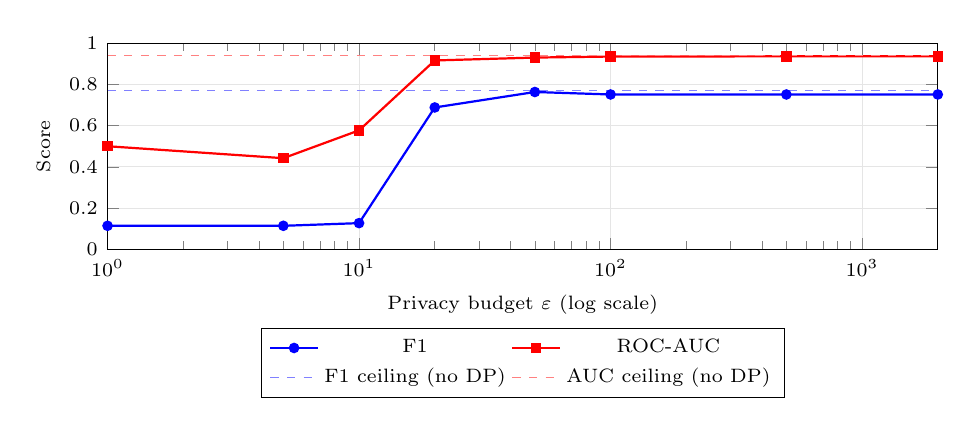
\begin{tikzpicture}
\begin{axis}[
    width=\columnwidth, height=4.2cm,
    xmode=log,
    xlabel={Privacy budget $\varepsilon$ (log scale)},
    ylabel={Score},
    ymin=0, ymax=1,
    xmin=1, xmax=2000,
    legend style={font=\scriptsize, at={(0.5,-0.38)}, anchor=north, legend columns=2},
    tick label style={font=\scriptsize},
    label style={font=\scriptsize},
    grid=major, grid style={gray!20},
]
\addplot[mark=*, mark size=1.5pt, blue, thick] coordinates {
    (1,0.114) (5,0.114) (10,0.127) (20,0.688) (50,0.763) (100,0.751) (500,0.751) (2000,0.751)
};
\addlegendentry{F1}
\addplot[mark=square*, mark size=1.5pt, red, thick] coordinates {
    (1,0.500) (5,0.442) (10,0.577) (20,0.916) (50,0.930) (100,0.935) (500,0.936) (2000,0.936)
};
\addlegendentry{ROC-AUC}
\addplot[dashed, blue!50!white] coordinates {(1,0.769) (2000,0.769)};
\addlegendentry{F1 ceiling (no DP)}
\addplot[dashed, red!50!white] coordinates {(1,0.938) (2000,0.938)};
\addlegendentry{AUC ceiling (no DP)}
\end{axis}
\end{tikzpicture}
\caption{Privacy-utility tradeoff from Table~\ref{tab:epsilon}: F1 and
ROC-AUC vs.\ $\varepsilon$. Dashed lines mark the no-DP ceiling.}
\label{fig:epsilon}
\end{figure}
\FloatBarrier

\subsection{Engineering Lessons: How the Numbers Got Trustworthy}
\label{sec:lessons}
We report three defects found and fixed during development, because
each one would have independently produced a misleadingly clean result
if left uncaught.

\textit{1) A trivially separable benchmark.} An early version of the
synthetic data generator drew fraud and legitimate transactions from
disjoint value ranges (e.g., legitimate amounts capped at \$400, every
fraud archetype starting above it). Every model, including a
RandomForest with no access to sequence structure, achieved 100\%
accuracy -- not because any model was good, but because the benchmark
was trivial. We rebuilt the generator with overlapping distribution
families and a 12\% ``quiet fraud'' fraction drawn from the legitimate
distribution.

\textit{2) An over-parameterized, collapsing model.} At
hidden\_dim=128 ($\approx1.07$M parameters for a 10-dimensional input),
the model would, under the harder benchmark, collapse to a constant
output (0\% recall, ROC-AUC exactly 0.5) once class imbalance and DP
noise were both present. We right-sized the architecture to
hidden\_dim=32 ($\approx45$K parameters), added a prior-informed bias
initialization (using the known fraud base rate), and a class weight
on the loss. This is also what dropped the usable DP $\varepsilon$
floor from $\sim$2000 down to $\sim$20--50, a $\sim$40--100$\times$
improvement, purely from right-sizing -- with no change to the privacy
mechanism itself, exactly as the $\sigma\sqrt{d}$ scaling in
Section~III-C predicts.

\textit{3) A NaN-masking bug hiding a real training failure.}
Guarding every loss term with a NaN-to-zero substitution prevented
crashes but let the model silently continue training on a degenerate,
input-ignoring prediction once corrupted, because
\texttt{contrastive\_loss} or \texttt{aux\_loss} evaluating to
\texttt{NaN} corrupted the total loss via \texttt{0.0 * NaN = NaN} even
at zero weight (IEEE~754 semantics). We fixed this by sanitizing
model outputs at their source rather than downstream, and by adding
per-round checkpoint-and-rollback so a round that does collapse cannot
poison the rest of training.

\section{Limitations}
\label{sec:limitations}
We report these plainly rather than rounding up. The original PaySim
dataset~\cite{lopezrojas2016paysim} is not available in our environment;
all reported numbers are on a schema-matched synthetic stand-in, useful
for pipeline correctness but not a real-world performance claim. The
graph branch is a simplified per-account encoder, not a relational
graph over shared entities (user, merchant, card, device), pending
real entity-linked edge data that our preprocessed sequence data does
not carry. Homomorphic encryption and secure aggregation are
implemented as correct reference code but are not exercised in the
live training loop reported here. All $\varepsilon$ values reported
are per-round budgets (Section~III-C); we do not report a formally
composed multi-round total, which would be strictly larger.

\section{Conclusion and Future Work}
We presented a federated, differentially private fraud detection
system and, more importantly, the measured evidence for its central
claim: that differential privacy has a real, quantifiable cost. The
honest comparison against the strongest non-private baseline
(centralized RandomForest; Table~\ref{tab:comparison}) is a gap of 0.8
percentage points of accuracy, and the clean, single-variable cost of
differential privacy itself (Table~\ref{tab:epsilon},
Fig.~\ref{fig:epsilon}) is approximately 1.8 F1 points at
$\varepsilon=100$ -- both in exchange for a formal privacy guarantee no
centralized or federated-without-DP baseline can offer. Future work
follows directly from Section~\ref{sec:limitations}: evaluating against
the original PaySim release, wiring homomorphic encryption and secure
aggregation into live training rather than leaving them as reference
implementations, extending the graph branch to real cross-account
entity links, applying a formal multi-round privacy accountant (e.g.,
R\'enyi DP composition) to report a total rather than per-round budget
(Section~III-C), and per-example gradient clipping (e.g.\ via Opacus)
to push the usable $\varepsilon$ floor lower without the
parameter-count penalty described in Section~III-C.

\section*{Acknowledgment}
The authors thank Dr. Prafullata Kiran Auradkar for guidance throughout
this project, and the Department of Computer Science and Engineering,
PES University.

\begin{thebibliography}{00}
\bibitem{mcmahan2017fedavg} H. B. McMahan, E. Moore, D. Ramage, S. Hampson, and B. A. y Arcas, ``Communication-Efficient Learning of Deep Networks from Decentralized Data,'' in \textit{Proc. 20th Int. Conf. Artificial Intelligence and Statistics (AISTATS)}, 2017, pp. 1273--1282.
\bibitem{li2020fedprox} T. Li, A. K. Sahu, M. Zaheer, M. Sanjabi, A. Talwalkar, and V. Smith, ``Federated Optimization in Heterogeneous Networks,'' in \textit{Proc. Machine Learning and Systems (MLSys)}, 2020.
\bibitem{mcmahan2018dp} H. B. McMahan, D. Ramage, K. Talwar, and L. Zhang, ``Learning Differentially Private Recurrent Language Models,'' in \textit{Proc. Int. Conf. Learning Representations (ICLR)}, 2018.
\bibitem{dwork2014dp} C. Dwork and A. Roth, ``The Algorithmic Foundations of Differential Privacy,'' \textit{Foundations and Trends in Theoretical Computer Science}, vol. 9, no. 3--4, pp. 211--407, 2014.
\bibitem{abadi2016dpsgd} M. Abadi, A. Chu, I. Goodfellow, H. B. McMahan, I. Mironov, K. Talwar, and L. Zhang, ``Deep Learning with Differential Privacy,'' in \textit{Proc. ACM SIGSAC Conf. Computer and Communications Security (CCS)}, 2016, pp. 308--318.
\bibitem{bonawitz2017secagg} K. Bonawitz, V. Ivanov, B. Kreuter, A. Marcedone, H. B. McMahan, S. Patel, D. Ramage, A. Segal, and K. Seth, ``Practical Secure Aggregation for Privacy-Preserving Machine Learning,'' in \textit{Proc. ACM SIGSAC Conf. Computer and Communications Security (CCS)}, 2017, pp. 1175--1191.
\bibitem{paillier1999} P. Paillier, ``Public-Key Cryptosystems Based on Composite Degree Residuosity Classes,'' in \textit{Proc. EUROCRYPT}, 1999, pp. 223--238.
\bibitem{lopezrojas2016paysim} E. A. Lopez-Rojas, A. Elmir, and S. Ahmed, ``PaySim: A Financial Mobile Money Simulator for Fraud Detection,'' in \textit{Proc. 28th European Modeling and Simulation Symposium (EMSS)}, 2016.
\bibitem{vaswani2017attention} A. Vaswani, N. Shazeer, N. Parmar, J. Uszkoreit, L. Jones, A. N. Gomez, L. Kaiser, and I. Polosukhin, ``Attention Is All You Need,'' in \textit{Proc. Advances in Neural Information Processing Systems (NeurIPS)}, 2017.
\bibitem{chen2020simclr} T. Chen, S. Kornblith, M. Norouzi, and G. Hinton, ``A Simple Framework for Contrastive Learning of Visual Representations,'' in \textit{Proc. Int. Conf. Machine Learning (ICML)}, 2020.
\end{thebibliography}

\end{document}
